\section{Proof, authority and applicable \$AGIALPHA utility}

\subsection{Four objects that must remain separate}

\textbf{WORLD} is the current mission: jobs, durations, capacity, releases, locks and the original evidence. \textbf{POLICY} is the executable dispatch, lookahead or repair strategy. \textbf{PROOF} is a current check against the frozen contract, with the checker identity and its independence limits. \textbf{AUTHORITY} is permission to perform a particular action now, under its scope, expiry and budget. An old observation can inform a new policy without validating the next result or authorizing its execution.

The unchanged released workbench returns research packs whose production admission is HOLD and whose independent-proof flag and authority grants remain unset. The new companion's independently implemented local check is recorded as research evidence alongside that pack; it does not rewrite the upstream production verdict. Import inspection yields historical evidence with empty active proof and authority. A browser history or copied archive therefore cannot promote itself into an operating grant \citep{montreal2026workbench1420}.

The research retained/incumbent decision throughout this paper concerns the finite experiment only. It is not a Harness release approval, native runtime admission or production authorization. The installed runtime, its signed journal, cycle CLI and preserved research scheduler were inspected separately. Native initialization would create local role credentials and was not performed. An unchanged source extension executed here is evidence for that extension, not for an installed four-product service.

\begin{figure}[ht]\centering
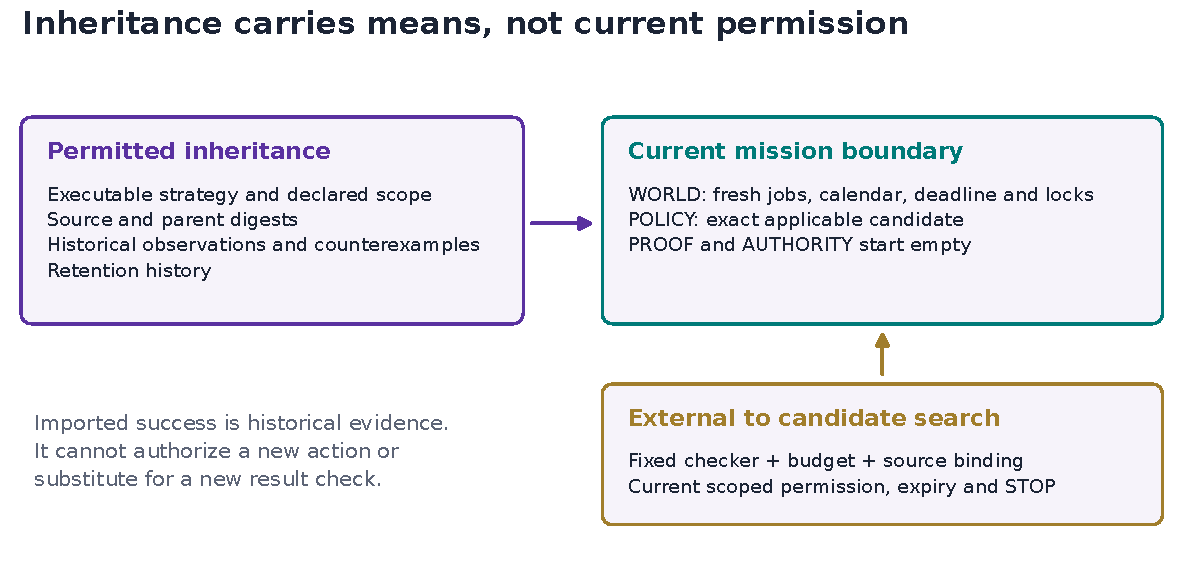
\includegraphics[width=\linewidth]{figures/proof-authority-boundary.pdf}
\caption{An artifact can cross generations with provenance. Current proof and action permission must be established separately.}\label{fig:authority}
\end{figure}

\subsection{Verified repository interfaces}

The source snapshot covers Alpha, Jobs, Manager and Fleet at the exact revisions listed in the evidence docket. Alpha's released v1.42.0 workbench provides the executed adapter seam and unchanged AGI Jobs draft compiler. Manager and Jobs expose \artifact{discoveryLabReceiverCapabilities}, \artifact{inspectDiscoveryLabWorkRequest} and \artifact{receiveDiscoveryLabWorkRequest}. Their inspected adapters report local inspection, no provisioned external submission and no production authority. Manager names a \artifact{USDC6} route; Jobs names an \artifact{AGIALPHA18} route. They are not a shared balance or an implicit currency conversion.

Fleet's inspected \artifact{SuccessorController} exposes prepare, execute, stop, result and health operations with principal, scope, expiry, runtime/policy binding and attempt limits. This study did not run that controller. Existing source-review and release restrictions remain in force. The paper supplies no evidence that those restrictions have been cleared.

\begin{table}[ht]\centering\small
\begin{tabularx}{\linewidth}{L{31mm}YY}
\toprule
Alpha contract & Source-verified relevant functions & Conditional practical purpose \\
\midrule
AscensionAccess & \artifact{register}, \artifact{owns}, \artifact{setAdmission}, \artifact{admitted}, \artifact{eligible} & Bind live ENS role ownership to a separate expiring admission. \\
NovaSeed & \artifact{seal}, \artifact{plan}, \artifact{creatorOf} & Commit a capsule hash, job-plan root, evidence hash and optional ancestry. \\
AscensionRiskOracle & \artifact{deposit/withdraw}, \artifact{lockForJob}, \artifact{openReview}, \artifact{attest}, \artifact{green} & AGIALPHA-denominated validator stake/capacity and result-bound review rounds. \\
AscensionJobMarket & \artifact{post/postFromSeed}, \artifact{bid}, \artifact{award}, \artifact{submit}, \artifact{validate}, \artifact{timeout}, \artifact{claimRefund} & Bounded work escrow, worker bonds, selected review, settlement or refund. \\
AscensionMark & \artifact{open}, \artifact{quote}, \artifact{buy/sell}, \artifact{transferLots}, \artifact{bloom}, \artifact{route}, \artifact{collect}, \artifact{close}, \artifact{reclaim} & Admitted funding lots and treasury-bounded routing of committed jobs. \\
\bottomrule
\end{tabularx}
\caption{Actual source interfaces at released Alpha commit \artifact{c352bad0}. Full paths, source copies and hashes are included \citep{alphaAscensionSource2026}. This table establishes source inspection only.}
\end{table}

\$AGIALPHA has a potential practical role when a separately commissioned work contract needs funded escrow, worker/validator commitments and attributable settlement. A sealed hash does not establish the underlying result's truth. Contract voting is not a scientific oracle. The demonstration is unsigned, unfunded and disconnected: no simulated contract execution, local EVM run, installed adapter submission or live settlement is claimed. Token issuance, reserve movements, scarcity and price appreciation are outside the productivity endpoint.

\subsection{Publication is another exact-source boundary}

Issue \href{https://github.com/MontrealAI/AGI-Alpha-Agent-v0/issues/4850}{\#4850} is the existing coordination surface \citep{alphaCoordination2026}. This work uses an isolated, additive research namespace and preserves all earlier editions. The receiving publication coordinator owns shared catalogue and deployment changes. Passive PDF publication and new interactive-source qualification are different gates. The final package provides exact artifact identities for that handoff; public links are reported only after retrieval and served-byte verification. No merge or deployment status is inferred from the existence of a local browser file.
